% Semantic Assistants - http://www.semanticsoftware.info/semantic-assistants
%
% This file is part of the Semantic Assistants architecture.
%
% Copyright (C) 2009, 2010, 2011 Semantic Software Lab, http://www.semanticsoftware.info
% The Semantic Assistants architecture is free software: you can
% redistribute and/or modify it under the terms of the GNU Affero General
% Public License as published by the Free Software Foundation, either
% version 3 of the License, or (at your option) any later version.
%   
% This program is distributed in the hope that it will be useful,
% but WITHOUT ANY WARRANTY; without even the implied warranty of
% MERCHANTABILITY or FITNESS FOR A PARTICULAR PURPOSE.  See the
% GNU Affero General Public License for more details.
% 
% You should have received a copy of the GNU Affero General Public License
% along with this program.  If not, see <http://www.gnu.org/licenses/>.

\chapter{Android Application}
Mobile phones use a variety of operating systems that transform them from a traditional handheld device for talking into general-purpose computing platforms. Android OS\footnote{Google's Android Platform~\url{http://developer.android.com}}, is an open source platform for mobile and tablet development led by Google Inc. It is a comprehensive Linux-based platform that supports most of the Java Platform and features its own extensive user interface framework. This platform is widely used by programmers to create applications and games for handheld devices. We have leveraged this platform to create an application that allows users to use novel NLP solutions inside their devices. This app, henceforth referred to as the \sa App, not only can be used as a standalone application, but also plays the role of a system-wide NLP service provider for other applications. Note that the \sa App was originally implemented based on Android 3.0 Platform\footnote{Android 3.0 Platform,~\url{http://developer.android.com/sdk/android-3.0.html}} (Honeycomb) but its backward compatibility has also been tested with Android 2.2. It is, however, recommended that the app be used in Android 3.0+ versions.

In the following sections, we describe the \sa App features and provide a guide on how to use the \sa App services inside external applications.

\section{Features}
The user interface shown in Figure~\ref{fig:android_main} is the \sa main activity (user interface). This means that once the app is installed on the device, this is the main entry to the application. It allows users to connect to a specific \sa server and invoke an assistant on the provided text input.

\begin{figure}[htb]
\centering
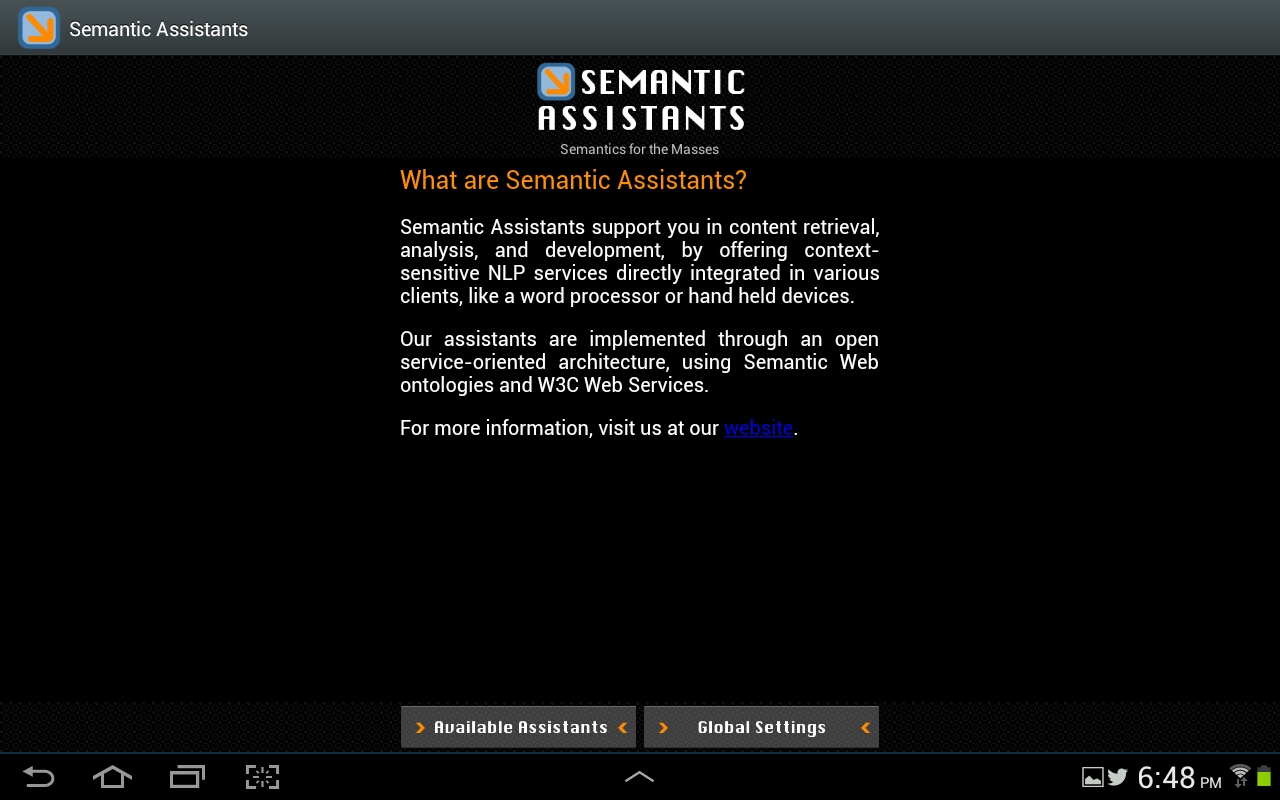
\includegraphics[scale=0.35]{pictures/android_main.jpg}
\caption{\sa Android App Main Activity}
\label{fig:android_main}
\end{figure}
\subsection{\sa Account}
Each android-enabled device has at least one built-in account type, i.e., the Google account. Android is designed in such a way that the same account can be registered to a variety of account-based services. For example, the Gmail account that is set up on the Android device is not just used for e-mailing , but for all the Google account-based applications. The same concept applies to the \sa App that uses the \emph{\sa account} type for its applications. Just like another accounts, you first need to sign up for a \sa Account before using the application.

Once you have obtained your credentials, on your device browse to \texttt{Settings $\rightarrow$ Accounts and Sync $\rightarrow$ Add Account} and choose the ``\sa'' option from the list. In the provided user interface, type in your \sa accounts credentials and press \texttt{Sign in}. If authenticated successfully, your \sa account will appear in the list of your device accounts.

\blankline
\noindent
\textbf{Note:} Before authenticating or signing up for an account, you need to choose the \sa server where your account is located. For this, follow the instructions in Section~\ref{sec:android_global_settings}.

\subsection{Global Settings}
\label{sec:android_global_settings}
Similar to other \sa clients, the \sa App allows users to connect to various arbitrary servers to inquire about their available assistants. On the \sa App main activity, press the \texttt{Global Settings} button. The application settings activity will pop up that allows you to define a new server location or choose one from a list of available servers as shown in Figure~\ref{fig:android_global_settings}.

\begin{figure}[htb]
\centering
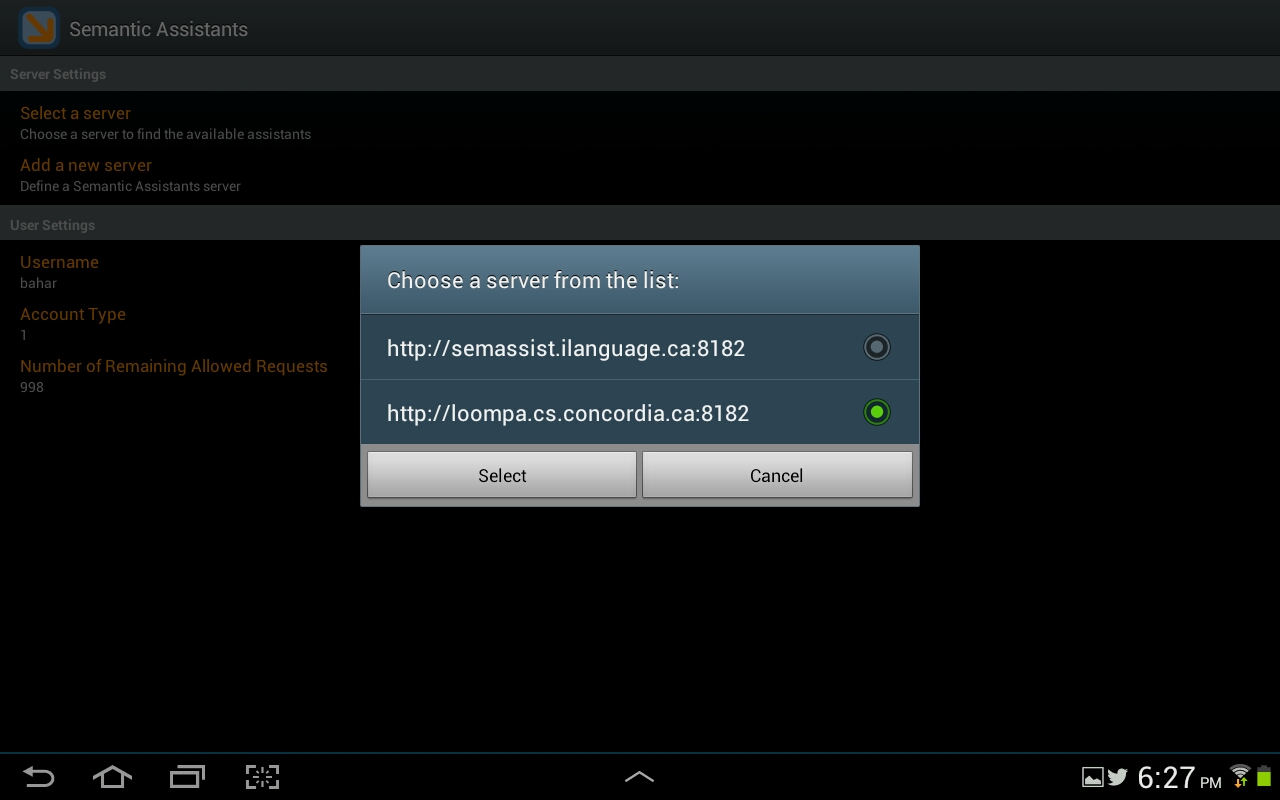
\includegraphics[scale=0.35]{pictures/android_global_settings.jpg}
\caption{\sa App Global Settings Activity}
\label{fig:android_global_settings}
\end{figure}

In order to add a new server location, click on the \texttt{Add a new server} option and type in the server URL by concatenating the server address, including its protocol and port number, like in Figure~\ref{fig:android_new_server}. In order to choose the newly defined server, choose the \texttt{Select a server} option from the Global Settings activity and select it from the list.

\begin{figure}[htb]
\centering
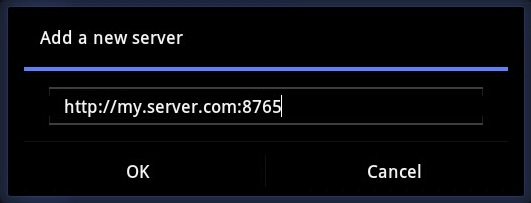
\includegraphics[scale=0.5]{pictures/android_new_server.jpg}
\caption{Adding a new server to the \sa App settings}
\label{fig:android_new_server}
\end{figure}

\subsection{NLP Service Invocation}
Once the \sa server is selected from the Global Settings activity, users can inquire about its available assistants. From the \sa App main activity, press the \texttt{Available Assistants} button to open the service invocation activity. This activity, as shown in Figure~\ref{fig:android_invoke_main}, presents the list of available assistants and an input text area for the text to be analyzed. By selecting each assistants from the list, the app will provide detailed information of what the assistant does and allows to customize the pipeline execution through providing runtime parameters.

\begin{figure}[htb]
\centering
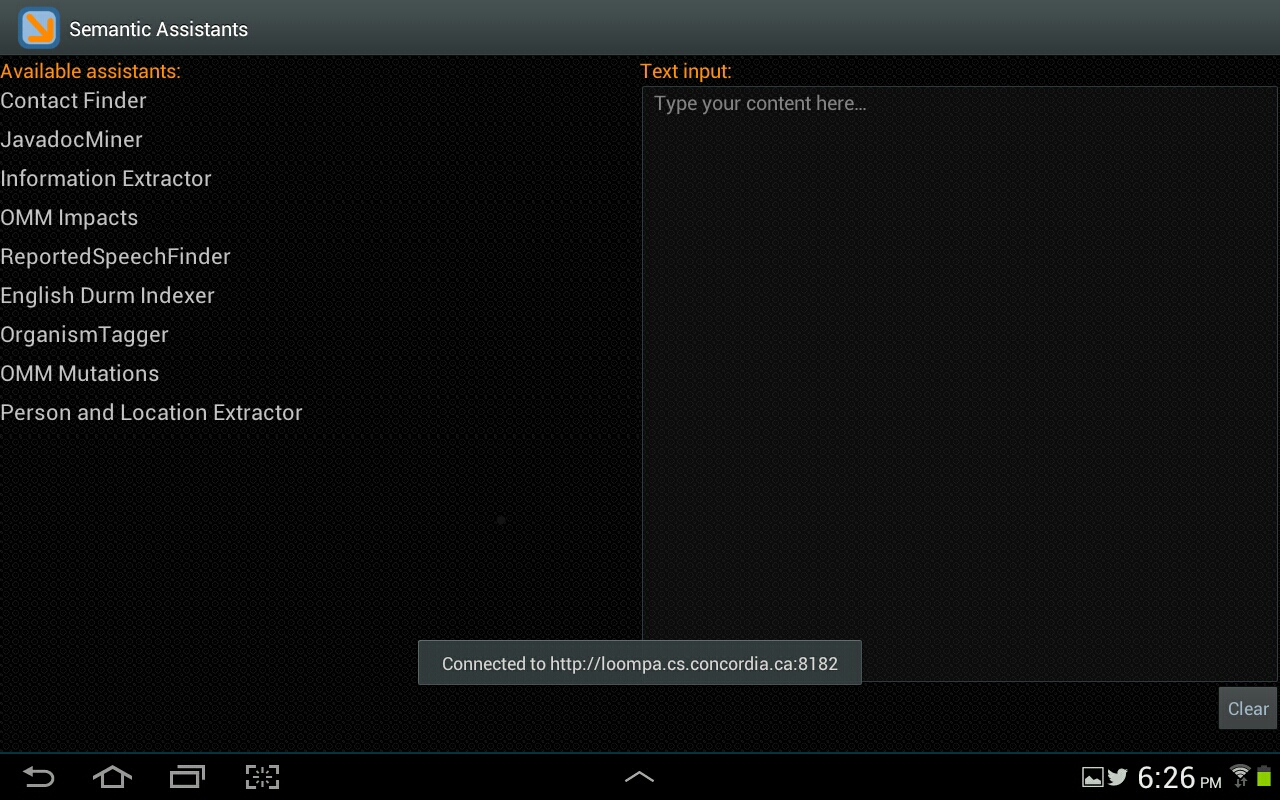
\includegraphics[scale=0.35]{pictures/android_invoke_main.jpg}
\caption{Invoking an NLP service through the \sa App settings}
\label{fig:android_invoke_main}
\end{figure}

Users have three options on how to provide a pipeline with text input:
\begin{itemize}
\item{\textbf{Manually typing in the text. }}{Using the device keyboard, type in the text that is to be analyzed.}
\item{\textbf{Sharing text with the \sa from other apps. }}{The \sa App listens for sharing event in the Android platform. This means that from within applications that provide a sharing mechanism, the selected text can be directly placed into the \sa Apps activity input.}
\item{\textbf{Sending input to the \sa service. }}{As we will explain more in Section \ref{sec:android_service}, the text input can be sent via a service argument (extra). The difference between this option and the previous bullet is that in the sharing option, the \sa App takes care of the result handling instead of the invoking application. Also in this service invocations, the NLP service to be executed is pre-defined and cannot be changed at a later stage.}
\end{itemize}
Once done with typing, select an assistants from the left-side list and press the \texttt{Invoke} button. Depending on the type of the results, you would either see the annotations in a new activity or the resulting file will be opened in the device browser.

\section{Installation}
TBD

\section{\sa App Service}
\label{sec:android_service}
As mentioned earlier, the \sa App also plays the role of a system-wide service provider, meaning that other external applications can use the \sa App's functionality. This is done through using Android services, i.e., application components that can perform long-running operations in the background. Each available service in the \sa App has a unique name that should be indicated when the external application invokes the service.

To better demonstrate this feature, we will illustrate a demo app that uses a \sa service. The demo in example, called iForgotWho, is an app that helps users to find potential ``contacts'' from a given text and upon user accept, automatically adds them to the device contact book. However, the iForgotWho app does not find the contacts by itself, rather it uses the \sa App's \texttt{person\_extractor} service. For this, the iForgotWho needs to (1) invoke the service using its complete identifier (available in the \sa App manifest file), (2) send along the text to be analyzed, and (3) indicate whether the \sa App should present the results or iForgotWho takes care of it. Once all the data is provided to the \sa App, the NLP service is executed and the results are passed back to iForgotWho app. Then, iForgotWho presented the list of all the person entities found in the text to the user, whom which ultimately decide whether they should be added to the device contact book. Figure~\ref{fig:android_service} illustrates this sequence.

\section{Development Notes}
In this section, we provide technical notes about the \sa App and how external Android application developers can integrate NLP capabilities in their apps using the \sa services.

\subsection{Extending the \sa App}
The \sa App source directory is structured as follows:
\begin{enumerate}
\item\url{activity}: This folder contains the classes representing graphical user interfaces.
\item\url{application}: This folder contains the \sa App's main application class and provides a static access to its context.
\item\url{business}: This folder contains the classes that handle communication with the \sa server.
\item\url{encryption}: This folder contains classes that take care of the secure HTTP connection attributes, such as the SSL certificate.
\item\url{intents}: This folder contains the intents factory class used by \sa App's services.
\item\url{parser}: This folder contains the parsers for Restful request and response representations.
\item\url{prefs}: This folder contains the utility classes for Android preference management.
\item\url{service}: This folder contains the authentication and service invocation service listeners.
\item\url{utils}: This folder contains the app's utility classes.
\end{enumerate}

In order to extend the \sa App, import the \sa App to your Eclipse or other IDE of choice. Note that you need to have the Android SDK\footnote{Android SDK, \url{http://developer.android.com/sdk/}} specific to your operating system installed on your machine.

\subsection{Using the \sa App Service}
In order integrate the \sa App service in your application, you have to first find the exact service name in the \sa App's manifest. For example, in order to detect Person named entities in a text, you have to call the \texttt{org.openintents.action.PERSON\_EXTRACTOR} service, using this code:

\begin{lstlisting}[language=Java,numbers=left,xleftmargin=4mm,columns=flexible]
 // specify which service should be invoked
 Intent service = new Intent(org.openintents.action.PERSON_EXTRACTOR);

 // the text to be analyzed
 String input = "I met John Smith at a conference last year.";

 // set the service input
 service.putExtra(Intent.EXTRA_TEXT, input);

 // let the Semantic Assistants App know the invoking app will present the results
 service.putExtra("SILENT_MODE", "true");

 // call the service
 startService(service);
\end{lstlisting}

You also have to define a Broadcast Receiver\footnote{Android Broadcast Receiver, \url{http://developer.android.com/reference/android/content/BroadcastReceiver.html}} to get back the results from the \sa App once the service results are ready. In your broadcast receiver class, you can then decide on how to present the results. Note that what the \sa App returns is the XML representation of the NLP pipeline as discussed in Section~\ref{sec:response}.

\subsection{Adding More ServiceIntents}
You can also easily add more services to the \sa App. In order to add a new service you must take the following steps:

\blankline
\noindent
\textbf{Step 1: Add the service name to list of available services. } In order to inform the \sa App of the newly added service, you need to add the unique name of the service as an \texttt{intent-filter} to the \texttt{service} node in the \sa App's manifest file. Specifically, you should add these lines to the \texttt{AndroidManifest.xml} file:

\begin{lstlisting}[language=XML,numbers=left,xleftmargin=4mm,columns=flexible]
<service android:name="info.semanticsoftware.semassist.android.service.SemanticAssistantsService"
		 android:process=":semassist_service" 
		 android:label="semassist">
	<intent-filter android:label="A_LABEL_FOR_YOUR_SERVICE">
		<action android:name="com.example.action.YOUR_SERVICE_NAME" />
		<category android:name="android.intent.category.DEFAULT" />
	</intent-filter>
</service>
\end{lstlisting}

Adding this line to the manifest allows the \sa App to receive the service requests from external applications.

\blankline
\noindent
\textbf{Step 2: Create the class that handles the results. }
Next is to create the class that will perform the actual service execution and handles the server response. This new class must extend the \texttt{ServiceIntent} class in the \texttt{intents} package and must have a \texttt{execute{}} method. In your execute method, you should let the parent class handle the actual service execution and instead handle the response before sending it back to the invoking app. The following snippet shows the service class for the \texttt{PERSON\_EXTRACTOR} service:

\begin{lstlisting}[language=Java,numbers=left,xleftmargin=4mm,columns=flexible]
public class PersonExtractorIntent extends ServiceIntent{

	// the exact service name as specified in its OWL file
	private final static String PR_NAME = "Person and Location Extractor";

	public PersonExtractorIntent(){
		super(PR_NAME);
	}

	public String execute() {
		//STEP1: Execute the service
		String rawResults = super.execute();

		//STEP2: Filter the results
		try{
			String filteredResult = "";
			// remove anything but "Person" annotations from the rawResults
			...
		} catch (Exception e){
			// handle exception
			....
		}
		return filteredResults
	}
}
\end{lstlisting}

\blankline
\noindent
\textbf{Step 3: Update the factory class. }
Finally let the \texttt{ServiceIntentFactory} class know how to map a service request to its corresponding handling class by adding the service action name to its enumeration class:

\begin{lstlisting}[language=Java,numbers=left,xleftmargin=4mm,columns=flexible]
/** Enumeration class for service intents */
enum Intents {person_extractor, YOUR_SERVICE_NAME};
\end{lstlisting}

\blankline
\noindent
and update the switch statement:

\begin{lstlisting}[language=Java,numbers=left,xleftmargin=4mm,columns=flexible]
switch(Intents.valueOf(action.toLowerCase())){
	case person_extractor:
		return new PersonExtractorIntent();
	case your_service_name
		return new YourServiceIntent();
	default:
		return null;
	}
\end{lstlisting}
